\documentclass[11pt]{article}
\input{/Users/markwang/.preamble}

\newcommand{\bbeta}{\boldsymbol{\beta}}
\newcommand{\bbetahat}{\boldsymbol{\hat{\beta}}}
\newcommand{\e}[1]{\mathbb{E} \{#1\}}
\newcommand{\bvar}[1]{\boldsymbol{\sigma^2}\{#1\}}
\newcommand{\bevar}[1]{\matr{s}^2\{#1\}}


\begin{document}


\section*{Chapter 6 Multiple Regression I}

\subsection*{
    \href[page=248]{../apply_linear_model_kutner.pdf}{6.1} Multiple Regression Models}

\begin{enumerate}
    \item \textbf{Need for Several Predictor Variables} A single predictor is often inadequate since often multiple variables affect the response variable in important and distinctive ways, this is especially true for observational experiments where predictor variables are not controlled. Even in controlled experiments, we often want to investigate a number of predictor variables simultaneously 
    \item \textbf{First-Order Model with Two Predictor Variables} A first order model is linear in predictor variables. A first-order model with 2 predictor variable is given by 
    \[
        Y_i = \beta_0 + \beta_1 X_{i1} + \beta_2 X_{i2} + \epsilon_i
    \]
    with regression function as
    \[
        \E\{ Y \} = \beta_0 + \beta_1 X_1 + \beta_2 X_2 
    \]
    A regression function in multiple regression is called a \textbf{regression surface} or a \textbf{response surface}. Parameter $\beta_1$ indicates the change in mean response $\E\{Y\}$ per unit increase in $X_1$ when $X_2$ is held constant. Hence, effect of $X_1$ on mean does not depend on levels of $X_2$, and vice versa, the predictor variables are said to have \textbf{additive effects}or \textbf{not to interact}. Paramters $\beta_1$ and $\beta_2$ are called \textbf{partial regression coefficients} since they reflect on partial effect of one predictor variable when other predictor variables is included in the model and is held constant. 
    \[
        \frac{\partial \E\{Y\}}{\partial X_1} = \beta_1 
        \quad \quad 
        \frac{\partial \E\{Y\}}{\partial X_2} = \beta_2
    \]
    \item \textbf{First-order model with More Than Two Predictor Variables} Consider $p-1$ predictor variables $X_1, \cdots, X_{p-1}$. A first-order model with $p-1$ predictor variables is given by
    \[
        Y_i = \beta_0 + \beta_1 X_{i1} + \beta_2 X_{i2} + \cdots + \beta_{p-1}X_{i, p-1} + \epsilon_i
    \]
    or equivalently
    \[
        Y_i = \beta_0 + \sum_{k=1}^{p-1} \beta_k X_{ik} + \epsilon_i
    \]
    Given $\E\{ \epsilon_i \} = 0$, the regression function is given by
    \[
        \E\{Y\} = \beta_0 + \beta_1 X_1 + \cdots + \beta_{p-1}X_{p-1}
    \]
    which represents a \textbf{hyperplane}. Parameter $\beta_k$ indicates change in the mean response $\E\{Y\}$ with a unit increase in predictor variable $X_k$, when all other predictor variables in the regression model are held constant
    \item \textbf{General Linear Regression Model} A general linear model, with normal error terms, is given by 
    \[
        Y_i = \beta_0 + \beta_1 X_{i1} + \beta_2 X_{i2} + \cdots + \beta_{p-1}X_{i, p-1} + \epsilon_i 
    \]
    where 
    \begin{enumerate}
        \item $\beta_0, \beta_1, \cdots, \beta_{p-1}$ are parameters 
        \item $X_{i1}, \cdots, X_{i, p-1}$ are known constants 
        \item $\epsilon_i$ are independent $\norm(0, \sigma^2)$
    \end{enumerate}
    with response function given by 
    \[
        \E\{Y\} = \beta_0 + \beta_1 X_1 + \beta_2 X_2 + \cdots + \beta_{p-1}X_{p-1} \tag{$\E\{\epsilon_i\}=0$}
    \]
    The general linear model usage cases
    \begin{enumerate}
        \item \textbf{$p-1$ Predictor Variables} as seen with first-order model with $p-1$ predictor variables, which has no interaction effects
        \item \textbf{Qualitative Predictor Variables} Indicator variables as $X_i$s. As an example of 1 quantitative predictor $X_{i1}$ and 1 indicator predictor variable $X_{i2}$
        \[
            \E\{Y\} = \beta_0 + \beta_1 X_1 + \beta_2 X_2 
        \]
        We have 2 response function 
        \[
            \E\{Y\} = \beta_0 + \beta_1 X_1 
            \quad \quad \quad 
            \E\{Y\} = (\beta_0 + \beta_2) + \beta_1 X_1
        \]
        which represents parallel straight lines with different intercepts. Generally we represents qualitative variable with $c$ classes by means of $c-1$ indicator variables 
        \item \textbf{Polynomial Regression} is a special case of generalized linear model contaiing higher-order terms of predictor variable, making the response function curlinear. For example 
        \[
            Y_i = \beta_0 + \beta_1 X_i + \beta_2 X_i^2 + \epsilon_i
        \]
        where $X_{i1} = X_i$ and $X_{i2} = X_i^2$
        \item \textbf{Transformed Variables}
        \item \textbf{Interaction Effects} When effects of predictor variables on response variable are not additive, the effect of one predictor variable depends on levels of other predictor variables. A \textbf{nonadditive regressfion model with 2 predictors $X_1$ and $X_2$} is given by 
        \[
            Y_i = \beta_0 + \beta_1 X_{i1} + \beta_2 X_{i2} + \beta_3 X_{i1}X_{i2} + \epsilon_i
        \]
        which is a special case of generalized linear model whereby $X_{i3} = X_{i1}X_{i2}$
        \item \textbf{Combination of above cases} For example, model that is curlinear with interaction terms.
        \item \textbf{Meaning of linear in General Linear Regression Model} Note GLM does is not restricted to linear response surfaces. \textbf{Linear Model} refers to the fact that model is linear in the parameters; it does not refer to the shape of the response surface. 
        \[
            Y_i  =\beta_0 exp(\beta_1 X_i) + \epsilon
        \]
        is a nonlinear regression model 
    \end{enumerate}
\end{enumerate}




\subsection*{
    \href[page=256]{../apply_linear_model_kutner.pdf}{6.2-6.6} General Linear Regression Model in Matrix Terms} 


\begin{enumerate}
    \item \textbf{GLR Model in Matrix} \\
    Given 
    \[
        \underset{n\times 1}{\matr{Y}} = 
        \begin{bmatrix}
            Y_1 \\ Y_2 \\ \vdots \\ Y_n \\ 
        \end{bmatrix}
        \quad 
        \underset{n\times p}{\matr{X}} = 
        \begin{bmatrix}
            1 & X_{11} & X_{12} & \cdots & X_{1, p-1} \\ 
            1 & X_{21} & X_{22} & \cdots & X_{2, p-1} \\ 
            \vdots & \vdots & \vdots & & \vdots \\
            1 & X_{n1} & X_{n2} & \cdots & X_{n, p-1} \\ 
        \end{bmatrix}
        \quad 
        \underset{p\times 1}{\beta} = 
        \begin{bmatrix}
            \beta_0 \\ \beta_1 \\ \vdots \\ \beta_{p-1} \\ 
        \end{bmatrix}
        \quad 
        \underset{n\times 1}{\epsilon} = 
        \begin{bmatrix}
            \epsilon_1 \\ \epsilon_2 \\ \vdots \\ \epsilon_n
        \end{bmatrix}
    \]
    The model is given by 
    \[
        \matr{Y = X\boldsymbol{\beta} + \boldsymbol{\epsilon}}
    \]
    where
    \[
        \underset{n\times n}{\matr{\sigma^2\{\boldsymbol{\epsilon}\}}} = 
        \begin{bmatrix}
            \sigma^2 & 0 & \cdots & 0 \\
            0 & \sigma^2 & \cdots & 0 \\
            \vdots & \vdots & & \vdots \\
            0 & 0 & \cdots & \sigma^2 \\ 
        \end{bmatrix}
        = \sigma^2 \matr{I}
    \]
    So the expectation of response given by 
    \[
        \E\{Y\} =  \matr{X\boldsymbol{\beta}} \quad \quad \matr{\sigma^2\{Y\}} = \sigma^2 \matr{I}
    \]
    \item \textbf{Estimation of Regression Coefficients} \\
    Idea is to minimize least squared 
    \[
        Q = \sum_i^n (Y_i - \beta_0 - \beta_1 X_{i1} - \cdots - \beta_{p-1}X_{i, p-1})^2
    \]
    minimize $Q$ to get normal equation 
    \[
        \matr{X'X\boldsymbol{\hat{\beta}} = X'Y}
    \]
    yielding least squared estimator 
    \[
        \boldsymbol{\hat{\beta}} = \matr{(X'X)^{-1}X'Y}
    \]
    \item \textbf{Fitted Values and Residuals} \\
    \begin{align*}
        \matr{\hat{Y}} &= \matr{X\boldsymbol{\hat{\beta}}} \\ 
        \matr{\hat{e}} &= \matr{(I-H)Y} \tag{where $\matr{H} = X(X'X)^{-1}X'$}  \\
        \e{\matr{\hat{e}}} &= 0 \\ 
        \bvar{\matr{\hat{e}}} &= \sigma^2\matr{(I-H)} \\ 
        \bevar{\matr{\hat{e}}} &= MSE(\matr{I-H}) \\ 
    \end{align*}
    \item \textbf{Sum of Squares and Mean Squares} \\
    Same as before 
    \begin{align*}
        SST &= \matr{Y'}\left[ \matr{I} - (\frac{1}{n})\matr{J} \right]\matr{Y}\\
        RSS &= \matr{Y'(1-H)Y}\\ 
        SSReg &= \matr{Y'}\left[ \matr{H} - (\frac{1}{n})\matr{J} \right]\matr{Y}\\
    \end{align*}
    with 
    \begin{enumerate}
        \item SST has $n-1$ degrees of freedom 
        \item RSS has $n-p$ degrees of freedom 
        \item SSReg has $p-1$ degrees of freedom
    \end{enumerate}
    So the mean square is given by
    \begin{align*}
        MSE = \frac{RSS}{n-p}
        \quad \quad 
        MSReg = \frac{SSReg}{p-1}
    \end{align*}
    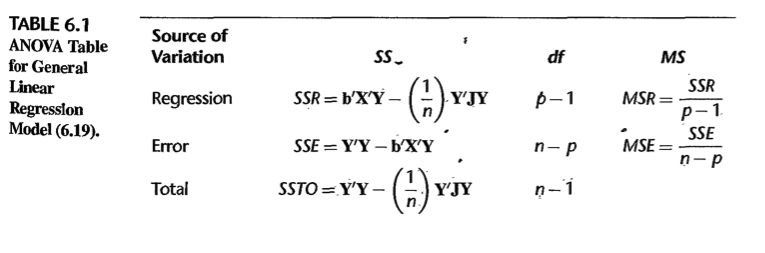
\includegraphics[width=\textwidth]{anova_table_for_GLR.png}
    \item \textbf{F-test for Regression Relation} tests for if there is a regression relation between the response variable $Y$ and the set of $X$ variable $X_1, \cdots, X_{p-1}$
    \[
        \begin{cases}
            \textsc{H}_0: \beta_1 = \beta_2 = \cdots = \beta_{p-1} = 0 \\
            \textsc{H}_{\alpha}: \text{ not all } \beta_{k} \text{ equal zero } k = 1, \cdots, p-1
        \end{cases}
    \]
    With test statistic 
    \[
        F&* = \frac{MSReg}{MSE}
    \]
    with 
    \[
        \begin{cases}
            \text{if } F^* \leq F_{1-\alpha, p-1, n-p} & \text{conclude } \mathsc{H}_0 \\
            \text{if } F^* > F_{1-\alpha, p-1, n-p} & \text{conclude } \mathsc{H}_{\alpha} \\
        \end{cases}
    \]
    When $p - 1 = 1$, test reduces to F test in SLR for if $\beta_1 = 0$
    \item \textbf{Coefficients of Multiple Determination} \\
    \[
        R^2 = \frac{SSReg}{SST} = 1 - \frac{RSS}{SST}
    \]
    which measures the proportionate reduction of total variation in $Y$ associated with the use of the set of $X$ variables. 
    \begin{enumerate}
        \item $R^2$ assumes value of 0 when $\hat{\beta}_k = 0$ for $k=1,\cdots, p-1$ and value 1 when all $Y$ observation fall directly on the fitted regression line 
        \item Adding more $X$ variables can only increase $R^2$ and never reduce it, because RSS can never become larger with more $X$ variables and SST is always the same for the given set of responses.
        \item \textbf{Adjusted coefficient of multiple determination} $R^2_{a}$ adjusts $R^2$ by dividing each sum of squares by its degree of freedom 
        \[
            R^2_{a} = 1 - \left( \frac{n-1}{n-p} \right)  \frac{RSS}{SST}
        \]
        $R^2_{a}$ may become smaller when another $X$ variable is introduced to the model. Since any decrease in $RSS$ maybe more than offset by the loss of a degree of freedom in the denominator $n-p$
        \item A large value of $R^2$ does not imply the fitted model is a useful one. For example, despite high $R^2$, fittedf model may not be useful if most predictions require extrapolation outside region of observations. Or if MSE may still be too large for inferences to be useful when high precision needed
    \end{enumerate}
    \item \textbf{Coefficient of Multiple Correlation} \\
    \[
        R = \sqrt{R^2}    
    \]
    \item \textbf{Inferences about Regression Parameters} \\
    Least squared and MLE estimators in $\hat{\beta}$ are unbiased
    \[
        \e{\bbetahat}  = \bbeta
    \]
    \[
        \bvar{\bbetahat} = \sigma^2 \underset{p\times p}{\matr{(X'X)}}^{-1}
    \]
    \[
        \bevar{\bbetahat} = MSE \underset{p\times p}{(\matr{X'X})}^{-1}
    \]
\end{enumerate}




\subsection*{
    \href[page=266]{../apply_linear_model_kutner.pdf}{6.8} Diagnostics and Remedial Measures}
    

\begin{enumerate}
    \item \textbf{Scatter Plot Matrix} \\
    $Y$ variable is found in its row, and $X$ variable is name found in the column \\ 
    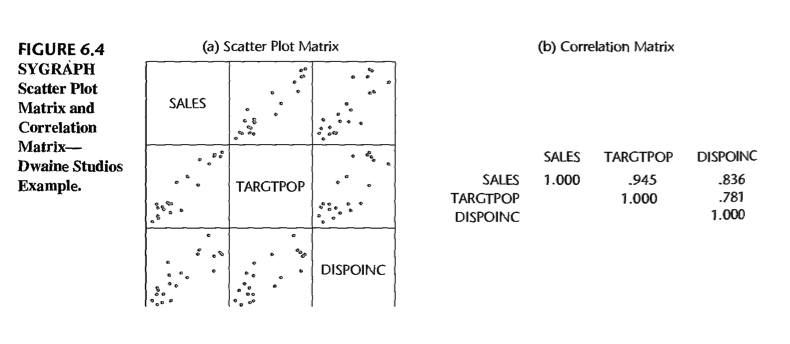
\includegraphics[width=\textwidth]{scatter_plot_matrix.png} \\
    First column we can compare plots of different predictor variables $X_i$ with $Y$. 
    \item \textbf{Correlation Matrix} \\
    contains coefficients of simple correlation $r_{Y,1}$, $r_{Y,2}$, $\cdots$, $r_{Y,p-1}$ between $Y$ and each of the predictor variables, and coefficients of simple correlation among predictor variables $r_{1,2}$ between $X_1$ and $X_2$
    \[
        \begin{bmatrix}
            1 & r_{Y,1} & r_{Y,2} & \cdots & r_{Y,p-1} \\ 
            r_{Y,1} & 1 & r_{1,2} & \cdots & r_{1,p-1} \\ 
            \vdots & \vdots & \vdots & & \vdots \\
            r_{Y,p-1} & r_{1,p-2} & r_{2,p-1} & \cdots & 1 \\ 
        \end{bmatrix}    
    \]
    which is symmetric with main diagonals containing 1s. Usually the first column/row is the response variable $Y$
    \item \textbf{Residual Plots} \\
    \begin{enumerate}
        \item Good for investigating constancy of variance of error terms, as well as for providing information about outliers.
        \item Residuals should be plotted against easch of the predictor variables, which provide informationa bout adequacy of the regression function w.r.t. that predictor variable.
        \item Should try plotting against important predictor variables omitted from the model.
    \end{enumerate}
    \item \textbf{Remedial Measures} \\
    Add a variable to account a curvature effect $X^2$ or interaction between $X_1$ and $X_2$ as $X_1 X_2$. Box-Cox transformation used to determine an appropriate power transformation on $Y$ for MLR. 
     
\end{enumerate}



\subsection*{
    \href[page=418]{../apply_linear_model_kutner.pdf}{10.1} Added-Variable Plots}

\begin{enumerate}
    \item \textbf{Motivation} Normal residual plot may not properly show nature of marginal effect of a predictor variable, given other predictor variables in the model. The added variable plot provides graphical information about the marginal importance of a predictor variable $X_k$, given the other predictor variables already in the model. 
    \item \textbf{Idea} Both response variable $Y$ and predictor variable $X_k$ under consideration are regressed against other predictor variables in the regression model and the residuals are obtained for each. 
\end{enumerate}
    




\subsection*{
    \href[page=312]{../apply_linear_model_kutner.pdf}{22} Multicollinearity and Its Effects}


\begin{enumerate}
    \item \textbf{Motivation} In nonexperimental situaitons, Predictor variables tend to be correlated among themselves and with other variables that are related to the response variable but are not included in the model
    \item \textbf{Multicollinearity} occurs when predictor variables are correlated among themselves. 
    \item \textbf{Uncorrelated Predictor Variables} predictor variable $X_1$ and $X_2$ are uncorrelated if coefficient of simple determination between the two are small, i.e. $r^2_{12} \sim 0$. When predictors are uncorrelated, their regression coefficients stay approximately the same regardless of any other uncorrelated predictors are in the model or not. Also, the marginal contribution of one predictor variable in reducing the error sum of squares when the other predictor variables are in the model is exactly the same as when this predictor variable is in the model alone. 
    \item \textbf{Problem with perfectly correlated predictor variables} If $X_1$ and $X_2$ are perfectly related, many different response function will lead to perfectly fitted values for the observation, and to the fitted values for any other $(X_1, X_2)$ combinations following the relation between $X_1$ and $X_2$. The response functions are not the same and will lead to different fitted values for $(X_1, X_2)$ combinations that do not follow the relation between $X_1$ and $X_2$
    \begin{enumerate}
        \item perfect correlation does not inhibit our ability to finda  good fit to data, or inferences about the mean respoinses or predictions of new observations 
        \item However, since many different response functions provide the same good fit, we cannot interpret any one set of regression coefficients as reflecting the effects of different predictor varaibles. This results in estimated regression coefficients having large sampling variability. We get different estimates of regression coefficients from one sample to the next. 
        \item We can no longer interpret a regression coefficients as measuring the change in the expected value of the response variable when the given predictor variable is increased by one unit while all other predictors are held constant. 
    \end{enumerate}
    \item \textbf{Effects of Multicollinearity} GIven scatter plot matrix and the correlation matrix of the predictor variables. 
    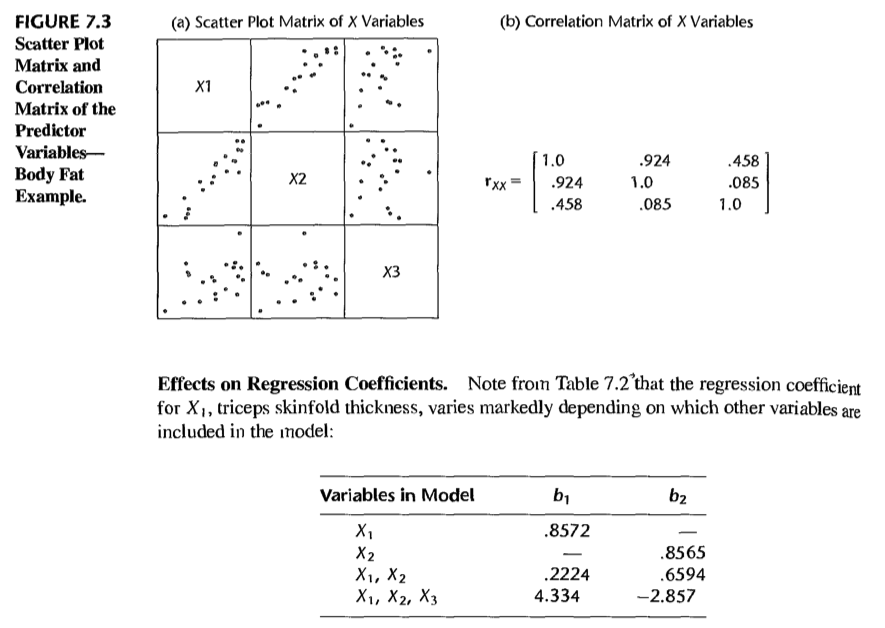
\includegraphics[width=\textwidth]{multicollinearity.png}
    Note $X_1$ and $X_2$ are highly correlated $r_{12} = 0.924$, $X_3$ is not highly correlated with $X_1$ and $X_2$ ($r_{13} = 0.458$, $r_{23} = 0.085$) but $X_3$ is highly correlated with $X_1$ and $X_2$ together by looking at coefficients of multiple determination. Note $\hat{\beta}_2$ changes sign when $X_3$ is added to the model that includes $X_1$ and $X_2$. 
    \begin{enumerate}
        \item \textbf{regression coefficients} Idea is when predictors are correlated, the regression coefficients of any one variable depends on which other predictors are included in the model and which one are left out. A regression coefficients does not reflect any inherent effect of the particular predictor variable on the response variable but only a marginal or partial effect.
        \item \textbf{sum of squares} marginal contribution of any one predictor varialbe in reducing error sum of squares varies, depending on which other variables are in th emodel. 
    \end{enumerate}
\end{enumerate}



\subsection*{
    \href[page=340]{../apply_linear_model_kutner.pdf}{22} Interaction Regression Models}






\subsection*{
    \href[page=951]{../apply_linear_model_kutner.pdf}{22} Analysis of Covariance}


\begin{enumerate}
    \item \textbf{ANCOVA} A special type of regression model, used for observational/designed studies. Idea is to augment ANOVA model. It is intended reduce variance of error terms in the model 
    \item \textbf{How ANCOVA reduce error variability} ANCOVA utilizes relationship between response variable and one or more quantitative variable for which the observations are available in order to reduce error term variability and make the study a more powerful one for comparing treatment effects. 
    \item \textbf{Concomitant (covariates) variable} Quantitative variable in covariance analysis is called concomitant variable. Concomitant variable usually has relationship with response variable. For example, age, status, aptitude in studying human subjects, etc. A concomitant variable should be observed before the study, or not be influenced by treatment in any way, if observed during the study, i.e. age. 
    \item When qualitative concomitant variable added, analysis of variance model where somer factors are of primary interest and others represent concomitant varaibles are included for purpose of error variance reduction 
\end{enumerate}


\newpage

\section*{
    \href[page=136]{../../modern_regression_r.pdf}{Chapter 5} Multiple Linear Regression}



\section*{
    \href[page=136]{../../modern_regression_r.pdf}{Chapter 5.2} Estimation and Inference in MLR}

\begin{enumerate}
    \item \textbf{Estimation and Inference in MLR} 
    \[
        \E\{ Y|X_1=x_1, X_2=x_2,\cdots,X_p=x_p \} = \beta_0 + \beta_1 x_1 + \cdots + \beta_p x_p 
    \]
    so 
    \[
        Y_i = \beta_0 + \beta_1 x_1 + \cdots + \beta_p x_p + e_i
    \]
    where $\E\{e_i | X\} = 0$, in which case response variable $Y$ is predicted from $p$ predictor varaibles $X_1,X_2,\cdots, X_p$
    \item \textbf{Least Squared matrix formation} 
    Regression model
    \[
        \matr{ Y = X\bbeta + e}    
    \]
    with $var(e) =\sigma^2\matr{I}$
    \[
        RSS(\beta) = \matr{(Y - X\bbeta)'(Y - X\bbeta)}
    \]
    Least square estimate given by
    \[
        \bbetahat = \matr{(X'X)^{-1}X'Y}    
    \]
    FItted value given by
    \[
        \matr{ \hat{Y} = X\bbetahat }
    \]
    \item \textbf{Least Squared Estimates properties}
    \[
        \matr{ \e{\bbetahat | X} = \bbeta } \quad \quad \quad \quad 
        Var(\bbetahat | X) = \sigma^2 \matr{(X'X)^{-1}}
    \]
    \item \textbf{Residual Sum of Squares}
    \[
        RSS =  \matr{(Y - X\bbeta)'(Y - X\bbeta)} = \matr{\hat{e}' \hat{e}} = \sum_i \matr{\hat{e}_i}^2 
    \]
    Error variance estimated by 
    \[
        s^2 = \frac{RSS}{n-p-1} = \frac{1}{n-p-1} \sum_i \matr{\hat{e}_i^2}    
    \]
    is an unbiased estimator of $\sigma^2$
    \item \textbf{Confidence interval and tests of significance} Assume normally distributed error with constant variance, it can be shown that for $i = 0, 1, \codts, p$, 
    \[
        T_i = \frac{ \hat{\beta}_i - \beta_i }{ se(\hat{\beta}) }  \sim t_{n-p-1}
    \]
    degree of freedom is difference between sample size and number of parameters estimated, i.e. $p+1$ for parameters $\beta_0, \beta_1, \cdots, \beta_p$
    \item \textbf{Adjusted $R^2$}
    \[
        R^2_{adj} = 1 - \frac{RSS / (n-p-1)}{SST / (n-1)}    
    \]
    \item \textbf{ANOVA to test linear association} 
    \[
        \begin{cases}
            \mathcal{H}_0 : \beta_1 = \cdots = \beta_p = 0 \\
            \mathcal{H}_{\alpha} : \text{ at least some of } \beta_i \neq 0 \\ 
        \end{cases}    
    \]
    \[
        F = \frac{SSreg / p}{ RSS / (n-p-1)}    
    \]
    $F$ has F distribution with $p$ and $n-p-1$ degrees of freedom when $H_0$ is true. F-test used to test for existence of a linear association between $Y$ and \textbf{ANY} of the $p$ x variable. If F-test is indeed significant then a natural question is to ask which of the $p$ x-variables is there evidence of a linear association with $Y$. We perform $p$ separate t-test $\mathcal{H}_0 : \beta_1 = 0$. However, there are problems interpreting results when predictors are highly correlated
    \item \textbf{Partial F-test} \\
    Test if a subset of predictors have regression coefficients equal to 0. 
    \[
        \begin{cases}
            \mathcal{H}_0 : \beta_1 = \cdots = \beta_k = 0 \text{ where } k < p & 
            \text{ reduced model }  Y = \beta_0 + \beta_{k+1}x_{k+1} + \cdots + \beta_p x_p + e \\
            \mathcal{H}_{\alpha} : \mathcal{H}_{0} \text{ not true } & 
            \text{ full model } Y = \beta_0 + \beta_1 x_1 + \cdots + \beta_p x_p + e \\ 
        \end{cases}    
    \]
    \[
        F = \frac{ (RSS_{reduced} - RSS_{full} ) / (df_{reduced} - df_{full}) }{ RSS_{full} / df_{full} }
        = \frac{ (RSS_{reduced} - RSS_{full} ) / k }{ RSS_{full} / (n-p-1) }
    \]
    Note, the reduced model includes all variable currently of interest except whose statistical significance we wish to test. Intuitively, we look at the average difference in RSS between 2 models and compare this to average predictor error in the best model we have (the full model). If error are roughly the same for two models, then the added regressors in the full model are not contributing a lot. But if average decrease in prediction error duer to added regressor is quite large, then the regressors are contributing a good deal of explanatory power and thus should be retained.
\end{enumerate}



\section*{
    \href[page=136]{../../modern_regression_r.pdf}{Chapter 5.3} Analysis of Covariance}


\begin{enumerate}
    \item \textbf{Analysis of Covariance} Naievely, ANOVA model has predictor variables that is quantitative (x) and qualitative (d). 
    \item \textbf{Coincident regression lines} The dummy variable $x$ has no effect on $Y$ 
    \[
        Y = \beta_0 + \beta_1 x + e
    \]
    \item \textbf{Parallel regression lines} Dummy varaible produces an additive change in $Y$
    \[
        Y = \beta_0 + \beta_1 x + \beta_2 d + e = 
        \begin{cases}
            \beta_0 + \beta_1 x + e & d = 0 \\
            \beta_0 + \beta_2 + \beta_1 x + e & d = 1\\ 
        \end{cases}    
    \]
    \item \textbf{Regression line with equal intercepts but different slopes} Dummy variabler only changes the size of the effect of $x$ on $Y$, that is, 
    \[
        Y = \beta_0 + \beta_1 x + \beta_3 d \times x + e = 
        \begin{cases}
            \beta_0 + \beta_1 x + e & d = 0 \\
            \beta_0 + (\beta_1 + \beta_3) x + e & d = 1 \\ 
        \end{cases}    
    \]
    \item \textbf{Unrelated regression lines} Dummy variable produces an additive change in $Y$ and also changes the size of effect of $x$ on $Y$ 
    \[
        Y = \beta_0 + \btea_1 x + \beta_2 d + \beta_3 d \times x + e = 
        \begin{cases}
            \beta_0 + \beta_1 x + e & d = 0 \\ 
            \beta_0 + \beta_2 + (\beta_1 + \beta_3)x + e & d = 1 \\ 
        \end{cases}  
    \]
\end{enumerate}





\section*{
    \href[page=161]{../../modern_regression_r.pdf}{Chapter 6} Diagnostics and Transformation for MLR} 


\section*{
    \href[page=161]{../../modern_regression_r.pdf}{Chapter 6.1} Regression Diagnostics for Multiple Regression}
    
    
\begin{enumerate}
    \item Determine if proposed regression model is valid by looking at \textbf{standardized residuals} plot 
    \item Determine if any data points are \textbf{leverage point} (with large effect on model) 
    \item Determine if any data points are \textbf{outliers}
    \item Assess effect of each predictor variable on the response variable, having adjusted for the effect of other predictors using \textbf{added variable plots}
    \item Assess extent of \textbf{collinearity} among predictor variables using \textbf{variance inflation factors}
    \item Examine if assumption of constant error variance is valid, 
    \item For time series data, examine if data are correlated over time
\end{enumerate}


\begin{enumerate}
    \item \textbf{Leverage Points} 
    \[
        \matr{Y = X \bbetahat = X(X'X)^{-1}X'Y = HY} 
        \quad \quad 
        \matr{H = X(X'X)^{-1}X'}    
    \]
    To classify $i$-th point as poitn of high leverage, in MLR model with $p$ predictors if 
    \[
        h_{ii} > 2 \times avg(h_{ii}) = 2 \times \frac{(p+1)}{n}
    \]
    \item \textbf{Standardized residuals} 
    \[
        \matr{\hat{e} = Y - \hat{Y} = (I - H)Y}    
    \]
    \[
        \e{\matr{\hat{e} | X}} = 0
    \]
    \[
        Var\{ \matr{\hat{e} | X} \} = \sigma^2(\matr{I-H})
    \]
    The $i$-th residual has variance given by 
    \[
        Var(\hat{e}_i) = \sigma^2\left[ 1 - h_{ii} \right]    
    \]
    The $i$-th standardized residual is given by 
    \[
        r_i = \frac{\hat{e}_i}{s \sqrt{1 - h_{ii}}} 
        \quad \quad \quad 
        s = \sqrt{\frac{\sum_j \hat{e}_j^2 }{n - (p+1)}} \text{ estimates } \sigma
    \]
    \item \textbf{Outlier} Points are outliers if the point falls outside interval from -2 to 2 for small datasets. 
    \item \textbf{Validity of Model} A MLR model is a valid model for the data if the conditional mean of $Y$ given $X$ is a linear function of $X$ and the conditional variance of $Y$ given $X$ is constant 
    \[
        \e{Y | X = x} = \beta_0 + \beta_1 x_1 + \beta_2 x_2 + \cdots + \beta_p x_p 
        \quad \quad 
        Var\{ Y| X=x \} = \sigma^2
    \]
    When a valid model has been fit, a plot of standardized residuals, $r_i$ against any predictor or any linear combination of predictors (i.e. response variable) will have properties
    \begin{enumerate}
        \item random scatter of points around horizontal axis, since mean function of $e_i$ is zero when a corrected model has been fit 
        \item Constant variability as we look along the horizontal axis 
    \end{enumerate}
    So any pattern in a plot of standardized residual is indicative that an invalid model has been fit to the data. 
    \item \textbf{Added variable plot} used to visually assess the effect of each predictor, having adjusted for the effects of the other predictors. It is simply a plot showing residual of response except $X_i$ against all predictors except $X_i$ vs. residual of $X_i$ on all other  predictors. This is mainly to overcome the shortcoming of plotting scatter plots of response variable against each of the predictor variable, which does not take into account the effect of the other predictor variable in the model where predictor variables are correlated (other variables are not held constant).  
    \begin{enumerate}
        \item Compute residuals of regressing response against predictor variables omitting $X_i$
        \item Compute residuals of regressing $X_i$ against the remaining independent variables 
        \item Plot residuals from 1 agaisnt residuals from 2
    \end{enumerate}
    It is used to identify outliers and heteroschedasticity. The slope in the plot is the partial regression coefficients. A linear pattern indicates that $X_i$ is useful in the model over and above other predictor variables, i.e. plot shows strengths of linear relationship $Y$ and $X_i$ over and above other variables. It is also useful for detecting nonlinear relationships, nonconstant variance, and influential points
    \item \textbf{Partial correlation} measures degree of association between 2 random variablers, with effect of the set of controlling random variables removed. Formally, partial correlation between $X$ and $Y$ given a set of $n$ controlling variables $\matr{Z} = \{ Z_1, \cdots, Z_n \}$ is the correlation between residfual $e_{X}$ and $e_{Y}$ resulting from the linear regressfion of $X$ with $\matr{Z}$ and of $Y$ with $\matr{Z}$
\end{enumerate}




\section*{
    \href[page=161]{../../modern_regression_r.pdf}{Chapter 6.4} Multicollinearity} 


\begin{enumerate}
    \item \textbf{Scenario} highly correlated data yields highly statistically significant F-test but very few of the regression coefficients may be statistically significant
    \item \textbf{Variance Inflation Factors} quantifies severity of multicollinearity. It provides an index that measures how much the variance (the square of the estimate's standard deviation) of an estimated regression coefficient is increased because of collinearity. It can be shown that 
    \[
        Var\{ \hat{\beta}_j \} = \frac{1}{1 - R_{j}^2} \times \frac{\sigma^2}{(n-1)s_{s_j}^2} 
        \quad \quad j = 1, \cdots, p
    \]
    variance inflation factor is given by 
    \[
        VIF = \frac{1}{1 - R_{j}^2}
    \]
    where $R_{j}^2$ denote value of coefficients of multiple correlation obtained from regression of $x_j$ on the other $x$s', i.e. amoutn of variability explained by this regression. 
    \item \textbf{Ridged Regression} 
    \[
        \bbetahat = \matr{(X'X + \lambda I)^{-1} X'Y}
    \]
    \item \textbf{Principle Component analysis} 
    \[
        \bbetahat = \matr{(Z'Z)^{-1} Z'Y}
    \]
    where $\matr{Z}$ is a lower dimension version of $X$
\end{enumerate}


\end{document}
